\section{Background}\label{sec:background}

It is commonly known that wireless systems communicating in the clear are vulnerable to signal overshadowing attacks.
However, performing these attacks in practice depends upon the physical layer and protocol properties of the overall system.
Existing work has explored similar techniques in areas such as WiFi deauthentication~\textbf{TODO: cite}, mobile internet~\cite{yang2019hiding,erni2021adaptover}, GNSS spoofing~\cite{tippenhauer2011requirements}, and even the instruments onboard aircraft~\cite{sathayeWireless2019}.
However, no existing work considers the vulnerability of Earth Observing satellite systems.

% Summarise currently deployed EO SATCOMs
% Summarise countermeasures

\subsection{Earth observing data link security}

Many Earth observing (EO) satellites face similar issues to other wireless systems which are built without robust cryptography at the data link.
These systems were built at a time when robust cryptography was uncommon due to less powerful onboard computers, and are still used in many applications including safety-critical infrastructure.

However unlike other wireless systems, satellites often produce useful data for decades after their launch, motivating current research into securing the communications without retrofitting cryptography.
Unlike relay satellite systems, EO satellites cannot be secured by upgrading only the groundstation endpoints.

Many unencrypted EO satellites exist; these include government satellite such as NASA's Earth Observing Fleet and NOAA's GOES fleet, alongside other CubeSats.
Other satellites use weak cryptography which can now be decrypted without knowledge of the key.
For example, the Korean satellite COMS-1 uses single DES encryption~\cite{lrit-key-dec}, which has led to customer keys being successfully extracted from satellite data.
Additionally, the GEO-KOMPSAT-2A satellite had its keys leaked on the Korea Meteorological Administration website, which to this day remain publicly available~\cite{xrit-rx}.

\subsection{Satellite derived data sets and use cases}

Data from EO systems are often processed into intermediate satellite-derived datasets (SDDs), which represent the raw data in a more accessible form, often within hours or less of the raw data being collected.
A growing market for specific purpose SDDs has emerged, including for forest fire monitoring~\cite{nasaFirms}, dust storm detection~\cite{sarikhani2021new}, and flood tracking~\cite{cloudToStreet}.
Table~\ref{tab:satellite-derived-datasets} summarizes a number of currently available satellite-derived datasets, which are derived from a mixture of self-operated, commercial, and open access satellites.

Where these SDDs depend upon satellite data derived from insecure data links, there is the capability for an attacker to manipulate the downstream systems.
% TODO: outline impact of a potential attacker

\subsection{Countermeasures}

To counteract these attacks, a number of countermeasures have been proposed to facilitate attack detection and offset the impact.
These attacks vary in effectiveness and complexity of implementation, allowing an organization to selectively implement some or all of them according to their attack surface and acceptable level of risk tolerance.

\subsubsection{Cryptographic measures}

The first and most obvious countermeasure is to simply encrypt downlinked signals using a cryptographic key known only to the operators, or alternatively to use cryptographic keys to sign the messages.
In both cases this makes it possible to verify that a message is legitimate and has not been tampered with.


\subsubsection{Multi-receiver data comparison}

\subsubsection{Timing analysis}

\subsubsection{Physical layer fingerprinting}

% TODO: insert diagram of common space comms protocols
% TODO: find out which other satellites are unencrypted, and especially those which are new and use CCSDS
% Are they generally encrypted above the CCSDS layer?

\begin{figure}
    \centering
    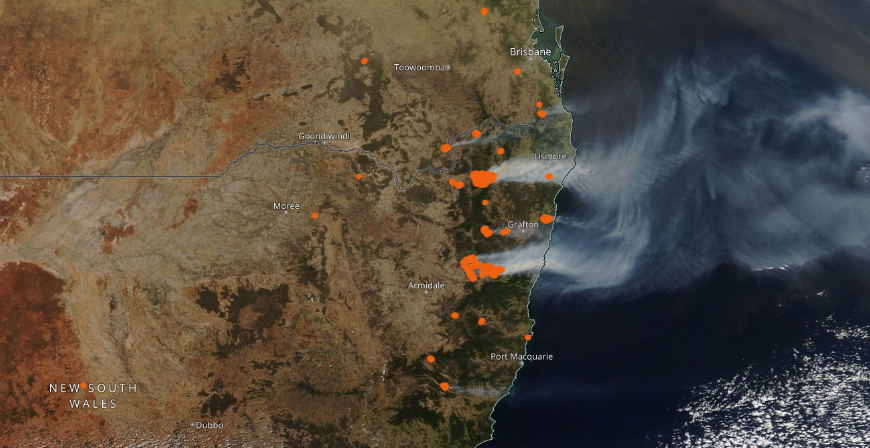
\includegraphics[width=\columnwidth]{diagrams/bushfire.png}
    \caption{The 2019 Australia bushfires as seen from Aqua's MODIS instrument, annotated with the \textit{Fires and Thermal Anomalies} dataset on NASA's worldview.\protect\footnotemark}
    \label{fig:bushfire}
\end{figure}

\footnotetext{Image taken from \url{https://worldview.earthdata.nasa.gov/?v=138.5214305912576,-37.663755528187544,165.90196079866635,-23.47436617591061\&as=2019-09-07-T00\%3A00\%3A00Z\&ae=2019-10-26-T16\%3A00\%3A00Z\&l=MODIS\_Combined\_Thermal\_Anomalies\_All,VIIRS\_SNPP\_Thermal\_Anomalies\_375m\_Day(hidden),VIIRS\_SNPP\_Thermal\_Anomalies\_375m\_Night(hidden),Reference\_Labels\_15m,Reference\_Features\_15m,Coastlines\_15m,VIIRS\_SNPP\_CorrectedReflectance\_TrueColor(hidden),MODIS\_Aqua\_CorrectedReflectance\_TrueColor,MODIS\_Terra\_CorrectedReflectance\_TrueColor(hidden)\&lg=false\&al=true\&av=3.5\&ab=on\&t=2019-09-07-T02\%3A00\%3A00Z}}


\begin{table*}
    \resizebox{\textwidth}{!}{%
    \begin{tabular}{lllll}
        \toprule
                     &       & \multicolumn{2}{c}{Satellites} & \\
        \cmidrule(lr){3-4}
        Organization & Usage & Provider & Nature & Data Access \\
        \midrule
        Planet Labs~\cite{planetProducts} & Various (intelligence, infrastructure, & Planet Labs & Self-operated & Commercial \\
                    & land use, water use) & & & \\
        Global Forest Watch~\cite{gfwMap} & Forest monitoring, carbon use, deforestation & Planet Labs & Commercial & Open access \\
        California Forest Observatory~\cite{cfoMap} & Monitoring forest fires in California & Planet Labs & Commercial & Open access \\
        ESRI~\cite{esriMap} & Land-use and land-cover maps & ESA (Sentinel-2) & Open access & Open access \\
        %Salo Sciences (TODO only bring back if I can say something about "forest restoration monitoring" project) & Conservation, climate monitoring & Planet Labs & Commercial & \\
        Meta~\cite{metaMap} & Population density maps & DigitalGlobe & Commercial & Open access \\
        Cloud to Street~\cite{cloudToStreet} & Flood tracking (disasters and insurance) & NASA (Terra/Aqua) & Open access & Commercial \\
        NCX Basemap~\cite{ncxBasemap} & Timber and carbon value monitoring in the USA & NASA & Open access & Commercial \\
        Upstream Tech HydroForecast~\cite{hydroforecast} & Water flow and weather intelligence & NASA (Terra/Aqua) & Open access & Commercial \\
        NASA FIRMS~\cite{nasaFirms} & Fire detection and management & NASA (EOS) & Self-operated & Open access \\
        \bottomrule
    \end{tabular}
    }
    \caption{Information on a number of satellite-derived datasets, including the satellite providers used to source the data.}
    \label{tab:satellite-derived-datasets}
\end{table*}
